% Options for packages loaded elsewhere
% Options for packages loaded elsewhere
\PassOptionsToPackage{unicode}{hyperref}
\PassOptionsToPackage{hyphens}{url}
\PassOptionsToPackage{dvipsnames,svgnames,x11names}{xcolor}
%
\documentclass[
  letterpaper,
  DIV=11,
  numbers=noendperiod]{scrartcl}
\usepackage{xcolor}
\usepackage{amsmath,amssymb}
\setcounter{secnumdepth}{5}
\usepackage{iftex}
\ifPDFTeX
  \usepackage[T1]{fontenc}
  \usepackage[utf8]{inputenc}
  \usepackage{textcomp} % provide euro and other symbols
\else % if luatex or xetex
  \usepackage{unicode-math} % this also loads fontspec
  \defaultfontfeatures{Scale=MatchLowercase}
  \defaultfontfeatures[\rmfamily]{Ligatures=TeX,Scale=1}
\fi
\usepackage{lmodern}
\ifPDFTeX\else
  % xetex/luatex font selection
\fi
% Use upquote if available, for straight quotes in verbatim environments
\IfFileExists{upquote.sty}{\usepackage{upquote}}{}
\IfFileExists{microtype.sty}{% use microtype if available
  \usepackage[]{microtype}
  \UseMicrotypeSet[protrusion]{basicmath} % disable protrusion for tt fonts
}{}
\makeatletter
\@ifundefined{KOMAClassName}{% if non-KOMA class
  \IfFileExists{parskip.sty}{%
    \usepackage{parskip}
  }{% else
    \setlength{\parindent}{0pt}
    \setlength{\parskip}{6pt plus 2pt minus 1pt}}
}{% if KOMA class
  \KOMAoptions{parskip=half}}
\makeatother
% Make \paragraph and \subparagraph free-standing
\makeatletter
\ifx\paragraph\undefined\else
  \let\oldparagraph\paragraph
  \renewcommand{\paragraph}{
    \@ifstar
      \xxxParagraphStar
      \xxxParagraphNoStar
  }
  \newcommand{\xxxParagraphStar}[1]{\oldparagraph*{#1}\mbox{}}
  \newcommand{\xxxParagraphNoStar}[1]{\oldparagraph{#1}\mbox{}}
\fi
\ifx\subparagraph\undefined\else
  \let\oldsubparagraph\subparagraph
  \renewcommand{\subparagraph}{
    \@ifstar
      \xxxSubParagraphStar
      \xxxSubParagraphNoStar
  }
  \newcommand{\xxxSubParagraphStar}[1]{\oldsubparagraph*{#1}\mbox{}}
  \newcommand{\xxxSubParagraphNoStar}[1]{\oldsubparagraph{#1}\mbox{}}
\fi
\makeatother


\usepackage{longtable,booktabs,array}
\newcounter{none} % for unnumbered tables
\usepackage{calc} % for calculating minipage widths
% Correct order of tables after \paragraph or \subparagraph
\usepackage{etoolbox}
\makeatletter
\patchcmd\longtable{\par}{\if@noskipsec\mbox{}\fi\par}{}{}
\makeatother
% Allow footnotes in longtable head/foot
\IfFileExists{footnotehyper.sty}{\usepackage{footnotehyper}}{\usepackage{footnote}}
\makesavenoteenv{longtable}
\usepackage{graphicx}
\makeatletter
\newsavebox\pandoc@box
\newcommand*\pandocbounded[1]{% scales image to fit in text height/width
  \sbox\pandoc@box{#1}%
  \Gscale@div\@tempa{\textheight}{\dimexpr\ht\pandoc@box+\dp\pandoc@box\relax}%
  \Gscale@div\@tempb{\linewidth}{\wd\pandoc@box}%
  \ifdim\@tempb\p@<\@tempa\p@\let\@tempa\@tempb\fi% select the smaller of both
  \ifdim\@tempa\p@<\p@\scalebox{\@tempa}{\usebox\pandoc@box}%
  \else\usebox{\pandoc@box}%
  \fi%
}
% Set default figure placement to htbp
\def\fps@figure{htbp}
\makeatother


% definitions for citeproc citations
\NewDocumentCommand\citeproctext{}{}
\NewDocumentCommand\citeproc{mm}{%
  \begingroup\def\citeproctext{#2}\cite{#1}\endgroup}
\makeatletter
 % allow citations to break across lines
 \let\@cite@ofmt\@firstofone
 % avoid brackets around text for \cite:
 \def\@biblabel#1{}
 \def\@cite#1#2{{#1\if@tempswa , #2\fi}}
\makeatother
\newlength{\cslhangindent}
\setlength{\cslhangindent}{1.5em}
\newlength{\csllabelwidth}
\setlength{\csllabelwidth}{3em}
\newenvironment{CSLReferences}[2] % #1 hanging-indent, #2 entry-spacing
 {\begin{list}{}{%
  \setlength{\itemindent}{0pt}
  \setlength{\leftmargin}{0pt}
  \setlength{\parsep}{0pt}
  % turn on hanging indent if param 1 is 1
  \ifodd #1
   \setlength{\leftmargin}{\cslhangindent}
   \setlength{\itemindent}{-1\cslhangindent}
  \fi
  % set entry spacing
  \setlength{\itemsep}{#2\baselineskip}}}
 {\end{list}}
\usepackage{calc}
\newcommand{\CSLBlock}[1]{\hfill\break\parbox[t]{\linewidth}{\strut\ignorespaces#1\strut}}
\newcommand{\CSLLeftMargin}[1]{\parbox[t]{\csllabelwidth}{\strut#1\strut}}
\newcommand{\CSLRightInline}[1]{\parbox[t]{\linewidth - \csllabelwidth}{\strut#1\strut}}
\newcommand{\CSLIndent}[1]{\hspace{\cslhangindent}#1}



\setlength{\emergencystretch}{3em} % prevent overfull lines

\providecommand{\tightlist}{%
  \setlength{\itemsep}{0pt}\setlength{\parskip}{0pt}}



 


\KOMAoption{captions}{tableheading}
\makeatletter
\@ifpackageloaded{caption}{}{\usepackage{caption}}
\AtBeginDocument{%
\ifdefined\contentsname
  \renewcommand*\contentsname{Table of contents}
\else
  \newcommand\contentsname{Table of contents}
\fi
\ifdefined\listfigurename
  \renewcommand*\listfigurename{List of Figures}
\else
  \newcommand\listfigurename{List of Figures}
\fi
\ifdefined\listtablename
  \renewcommand*\listtablename{List of Tables}
\else
  \newcommand\listtablename{List of Tables}
\fi
\ifdefined\figurename
  \renewcommand*\figurename{Figure}
\else
  \newcommand\figurename{Figure}
\fi
\ifdefined\tablename
  \renewcommand*\tablename{Table}
\else
  \newcommand\tablename{Table}
\fi
}
\@ifpackageloaded{float}{}{\usepackage{float}}
\floatstyle{ruled}
\@ifundefined{c@chapter}{\newfloat{codelisting}{h}{lop}}{\newfloat{codelisting}{h}{lop}[chapter]}
\floatname{codelisting}{Listing}
\newcommand*\listoflistings{\listof{codelisting}{List of Listings}}
\makeatother
\makeatletter
\makeatother
\makeatletter
\@ifpackageloaded{caption}{}{\usepackage{caption}}
\@ifpackageloaded{subcaption}{}{\usepackage{subcaption}}
\makeatother
\usepackage{bookmark}
\IfFileExists{xurl.sty}{\usepackage{xurl}}{} % add URL line breaks if available
\urlstyle{same}
% fallback for those not using the hyperref driver hyperxmp:
\makeatletter
\@ifundefined{xmpquote}{\newcommand{\xmpquote}[1]{#1}}{}
\makeatother
\hypersetup{
  pdftitle={LLM-Assisted Close Reading},
  pdfauthor={Jasper Harrington; Michael Falk},
  colorlinks=true,
  linkcolor={blue},
  filecolor={Maroon},
  citecolor={Blue},
  urlcolor={Blue},
  pdfcreator={LaTeX via pandoc}}


\title{LLM-Assisted Close Reading}
\usepackage{etoolbox}
\makeatletter
\providecommand{\subtitle}[1]{% add subtitle to \maketitle
  \apptocmd{\@title}{\par {\large #1 \par}}{}{}
}
\makeatother
\subtitle{The `Aeolus' Episode of James Joyce's \emph{Ulysses}}
\author{Jasper Harrington \and Michael Falk}
\date{2026-11-13}
\begin{document}
\maketitle
\begin{abstract}
In this presentation, we report on our experiments performing
LLM-assisted close reading of the `Aeolus' episode of James Joyce's
\emph{Ulysses}. The aim is twofold: (1) to explore Joyce's use of media
discourse in the episode; (2) to develop rigorous, reproducible methods
for LLM-assisted close reading. For this initial presentation, we
explain our reproducible pipeline, initial experimental results,
validation of the LLM analysis against classic lexicon-based sentiment
analysis, and initial impressions of close reading one section of
`Aeolus' in the light of the results.
\end{abstract}


\section{Introduction}\label{introduction}

\textsubscript{Source:
\href{https://uom-digital-studies.github.io/aeolus-microtexts/index.qmd.html}{Article
Notebook}}

In this presentation, we report on our experiments performing
LLM-assisted close reading of the `Aeolus' episode of James Joyce's
\emph{Ulysses}. The `Aeolus' episode marks a crucial ``hermeneutic
shift'' in the novel (Lawrence 1980, 392). In prior episodes, the
novel's language is primarily transparent and referential, as Joyce
tries to create the illusion of a stream of consciousness; in `Aeolus',
new voices are introduced, in the form of newspaper headlines, which
interrupt the stream of consciousness and render the language opaque.
Who is speaking? Is there a consciousness behind the words? Where is the
divide between nature and artifice, between art and life? This
``hermeneutic shift'' continues in later episodes of the novel, as the
language becomes increasingly opaque and self-referential.

Our aims in this paper are twofold:

\begin{quote}
\textbf{Aim 1:} To try to discover new angles of interpretation with the
assistance of LLMs.

\textbf{Aim 2:} To try and determine best practices for open,
reproducible literary-critical research using LLMs.
\end{quote}

To pursue these aims, we choose to focus on ``mediatization'' in the
episode (Schneider 1989). The episode takes place in a newspaper office,
and the episode's key linguistic feature is the intrusion of newspaper
headlines that ironically label the action. We therefore analyse the
language of the episode as media discourse, using a traditional
text-analytic technique (lexicon-based sentiment analysis) and an
LLM-assisted analogue of this technique (LLM-based sentiment and
thematic analysis).

This abstract is a quarto notebook. Code for all figures and
calculations can be viewed
\href{https://uom-digital-studies.github.io/aeolus-microtexts/dh2027/index-preview.html}{on
the research compendium website}.

\section{Literature Review}\label{sec-lit-review}

Like all episodes of \emph{Ulysses}, `Aeolus' has been subject to
intense analysis. For this presentation, we survey the literature on
media discourse in `Aeolus'. In a classic article, McLuhan (1954) argues
that \emph{Ulysses} reflects the temporal rhythms of the news media.
Like a daily newspaper, Joyce's stream-of-consciousness technique
realises ``a continuous present for events past, present and future''
(1954, 46). McLuhan sees a deep harmony between the stream of
consciousness and media discourse in \emph{Ulysses}. Subsequent scholars
have reversed McLuhan's judgment. Lawrence (1980), Schneider (1989) and
Radak (2017) all argue that the newspaper headlines in `Aeolus' are
intrusive, and disrupt the stream of consciousness.

We build on these readings in two ways. First, we re-adjudicate the
dispute between McLuhan and his followers. Is it really true that the
headlines are intrusive and disruptive, or do they in fact split the
chapter into rational units? Second, we consider `mediatization' in a
new context, considering how the form of the chapter resonates with
contemporary social media.

To do this, we split `Aeolus' on the headlines, converting the episode
into 63 ``microtexts''. We study these microtexts as though they were
social media posts, to see if these reveals new patterns in the
language.

The principal analytic method we use is sentiment analysis, which was
originally developed for social media analysis, but has subsequently
become a crucial tool for plot analysis (Elkins 2022; Franta and Silver
2024; Kim 2022; Falk 2024, chap. 6). In this project, we draw on recent
research by Ornstein et al. (2025) and Mens and Gallego (2025) to
formulate a reproducible pipeline for LLM-based sentiment analysis, as
explained below. For comparison, we apply the afinn (Nielsen 2011), bing
(Hu and Liu 2004) and syuzhet (Jockers 2015) sentiment lexicons to
Aeolus for sentiment analysis, using Hutto and Gilbert (2014)'s method
for normalising the scores. As we explain in
Section~\ref{sec-methodology}, LLMs have caused an upheaval in sentiment
analysis, allowing much more context-sensitive data extraction at the
cost of reliability and interpretability.

\section{Methodology: The Reproducible Pipeline}\label{sec-methodology}

LLMs are powerful but flawed tools for text analysis. In our view,
existing practices of open, reproducible scholarship are already
sufficient to realise much of the power while mitigating the flaws.

LLMs are powerful primarily because of \emph{in-context learning} and
\emph{structured outputs}. In-context learning is a powerful technique
for controlling the LLM's response to data: the researcher provides
contextual clues in the prompt, enabling the LLM to respond more
sensitively to the input data (Ornstein et al. 2025, 269) Structured
outputs make the output easier to process, by ensuring that it conforms
to a provided json schema ({``Structured Model Outputs {\textbar}
{OpenAI} {API},''} n.d.). This does not prevent hallucinations, but does
ensure that data is uniformly formatted for processing.

They are flawed because they are inherently \emph{inexplicable} and
\emph{unreliable}. The problem of LLM explicability is well known
(Goebel et al. 2018). LLMs have billions or trillions of parameters that
defy interpretation. Existing models have no power of introspection,
meaning that they can never give genuine explanations of their own
actions. The problem of LLM unreliability has only recent been subject
to serious research (Barke and Murali 2026; Rabanser et al. 2026). Early
research is not promising: as LLMs have become more capable, they have
not been getting more reliable. Even as LLMs have become more capable,
their consistency, robustness, predictability, calibration and safety
have hardly improved (Rabanser et al. 2026).

To address these flaws, we adopt the following principles for our
pipeline:

\begin{enumerate}
\def\labelenumi{\arabic{enumi}.}
\tightlist
\item
  \emph{Run the analysis locally}: We use Ollama to run all LLM analysis
  locally, on NVidia A100 GPUS available on our University's HPC cluster
\item
  \emph{Set temperature to 0}: When temperature is set to 0, LLMs become
  deterministic, always giving the same output to the same prompt.
\item
  \emph{Systematically vary the prompt and data}: Rather than
  interacting with the LLM in a chat environment to determine which
  prompt will work, we systematically run the analysis with different
  prompts and data structures, to assess what difference they make.
\item
  \emph{Make the pipeline fully reproducible}: When we run a set of
  experiments, full data are recorded for inspection by other scholars.
  All experimental data and LLM orchestration code are stored in a
  research compendium in the form of an installable R package.
\item
  \emph{Evaluate LLM analysis against other approaches}: Since the aim
  of our project is LLM-assisted close reading, we evaluate the LLM
  analysis against our own close reading of the text, supplemented with
  traditional, well-understood text analytic techniques (so far,
  lexicon-based sentiment analysis).
\end{enumerate}

The data for the project is stored in a research compendium (Marwick et
al. 2018), available at
\url{https://uom-digital-studies.github.io/aeolus-microtexts}. The
compendium contains an R package with our orchestration code,
experimental data from all successful runs, and our manuscripts.

At the time of this abstract, one set of experimental data is available
in the package (Table~\ref{tbl-list-runs}).

\begin{longtable}[]{@{}
  >{\raggedright\arraybackslash}p{(\linewidth - 6\tabcolsep) * \real{0.2569}}
  >{\raggedright\arraybackslash}p{(\linewidth - 6\tabcolsep) * \real{0.1835}}
  >{\raggedright\arraybackslash}p{(\linewidth - 6\tabcolsep) * \real{0.1009}}
  >{\raggedright\arraybackslash}p{(\linewidth - 6\tabcolsep) * \real{0.4587}}@{}}

\caption{\label{tbl-list-runs}Available experimental `runs' in
\texttt{aeolusmicrotexts}}

\tabularnewline

\toprule\noalign{}
\begin{minipage}[b]{\linewidth}\raggedright
run\_id
\end{minipage} & \begin{minipage}[b]{\linewidth}\raggedright
date
\end{minipage} & \begin{minipage}[b]{\linewidth}\raggedright
version
\end{minipage} & \begin{minipage}[b]{\linewidth}\raggedright
models
\end{minipage} \\
\midrule\noalign{}
\endhead
\bottomrule\noalign{}
\endlastfoot
20261019-131523\_v0.2.0.9000 & 2026-10-19 13:15:23 & 0.2.0.9000 &
llama3.2:3b , llama3.3:70b , deepseek-v2:16b \\

\end{longtable}

\textsubscript{Source:
\href{https://uom-digital-studies.github.io/aeolus-microtexts/index.qmd.html}{Article
Notebook}}

The results are stored in a long, self-describing format, to make their
inspection and replication simpler for other scholars
(Table~\ref{tbl-result-schema}).

\textsubscript{Source:
\href{https://uom-digital-studies.github.io/aeolus-microtexts/index.qmd.html}{Article
Notebook}}

\begin{longtable}[]{@{}
  >{\raggedright\arraybackslash}p{(\linewidth - 2\tabcolsep) * \real{0.5000}}
  >{\raggedright\arraybackslash}p{(\linewidth - 2\tabcolsep) * \real{0.5000}}@{}}
\caption{Data schema for experimental
results}\label{tbl-result-schema}\tabularnewline
\toprule\noalign{}
\begin{minipage}[b]{\linewidth}\raggedright
column
\end{minipage} & \begin{minipage}[b]{\linewidth}\raggedright
meaning
\end{minipage} \\
\midrule\noalign{}
\endfirsthead
\toprule\noalign{}
\begin{minipage}[b]{\linewidth}\raggedright
column
\end{minipage} & \begin{minipage}[b]{\linewidth}\raggedright
meaning
\end{minipage} \\
\midrule\noalign{}
\endhead
\bottomrule\noalign{}
\endlastfoot
\texttt{research\_question} & Which research question is passed to the
LLM: one of \texttt{"sentiment"} \textbar{} \texttt{"nationalism"}
\textbar{} \texttt{"ugc"} \\
\texttt{model} & Name of the Ollama model that is passed to
\texttt{ollama\ pull}, e.g.~\texttt{"llama3.2:1b"} \\
\texttt{context\_variant} & Which contextual clue is passed to the LLM:
\texttt{"no\_context"} (no information about where the text comes from),
\texttt{"ulysses\_context"} (LLM is told the text is from
\emph{Ulysses}), \texttt{"media\_text\_context"} (LLM is told that the
text is social media text) \\
\texttt{granularity} & How `Aeolus' is tokenised; it is either split
into each \texttt{"microtext"}, or into each \texttt{"sentence"} \\
\texttt{include\_headlines} & boolean; whether the headlines should be
included in the corpus for analysis \\
\texttt{microtext} & Since the table has one row per unit, and each
microtext could be split into multiple sentences, each row is labelled
with the numeric id of each microtext. \\
\texttt{unit\_index} & Since each microtext may be split into a sub-unit
(the sentence), each row is labelled with a numeric index of the
sub-unit (if
\texttt{granularity\ ==\ \textquotesingle{}microtext\textquotesingle{}}),
this is always \texttt{1}, since each microtext consists of 1 unit
only. \\
\texttt{unit\_of\_analysis} & The exact text string sent to the LLM for
this row's classification call \\
\texttt{label} & The schema's enum classification,
e.g.~\texttt{"positive"}, \texttt{"neutral"} and \texttt{"negative"} for
the sentiment analysis schema. \\
\texttt{score} & The schema's numeric score, always between -1 and 1 \\
\end{longtable}

As part of our research compendium, we provide a utility allowing
researchers to see exactly how the LLM is prompted. Since we run the
LLMs locally, we have full control over the exact prompt: it appears
that cloud providers sometimes modify user prompts without warning.
Below, we give an example of a prompt that would be sent to Ollama (with
the microtext truncated for space). We gave three tasks to the LLMs. In
the body of this abstract, we discuss only the first task, sentiment
analysis. Other results are shown in Section~\ref{sec-other-rqs}.

\begin{verbatim}
------------------------------------------------------------
SYSTEM PROMPT (fixed instructions for experiment)
------------------------------------------------------------
This text is from James Joyce's novel Ulysses. Classify the
sentiment of this text as positive, neutral, or negative.

## Output fields

Respond with a JSON object containing these fields, in this
order.

### label
Overall sentiment of the text.
Allowed values: "positive", "neutral", "negative".

### score
Sentiment intensity, from -1 (most negative) to 1 (most
positive).
Type: number.
------------------------------------------------------------
USER TURN (datum for analysis)
------------------------------------------------------------
## The text

 DEAR DIRTY DUBLIN

Dubliners.

—Two Dublin vestals, Stephen said, elderly and pious,
have lived fifty and fiftythree years in Fumbally’s lane.
[...]
------------------------------------------------------------
JSON SCHEMA (constrains output; not seen by model)
------------------------------------------------------------
{
  "type": "object",
  "description": "Classify the sentiment of this text as
  positive, neutral, or negative",
  "properties": {
    "label": {
      "type": "string",
      "description": "Overall sentiment of the text",
      "enum": ["positive", "neutral", "negative"]
    },
    "score": {
      "type": "number",
      "description": "Sentiment intensity, from -1 (most
      negative) to 1 (most positive)"
    }
  },
  "required": ["label", "score"],
  "additionalProperties": false
}
\end{verbatim}

\textsubscript{Source:
\href{https://uom-digital-studies.github.io/aeolus-microtexts/index.qmd.html}{Article
Notebook}}

\section{Initial Results}\label{sec-initial-results}

Our initial experiments were constrained by the software available on
our local HPC cluster. An old version of Ollama was installed, meaning
only certain models were available. Initial results are shown in
Figure~\ref{fig-microtext-granularity} and
Figure~\ref{fig-sentence-aggregation}. For the experiments shown in
Figure~\ref{fig-microtext-granularity}, the LLM was prompted with the
entire microtext each time, and asked to provide an overall label and
score. For Figure~\ref{fig-sentence-aggregation}, the LLM graded each
sentence separately, and then the labels and scores were averaged for
each microtext.

\textsubscript{Source:
\href{https://uom-digital-studies.github.io/aeolus-microtexts/index.qmd.html}{Article
Notebook}}

\protect\phantomsection\label{cell-fig-microtext-granularity}
\begin{figure}[H]

\centering{

\pandocbounded{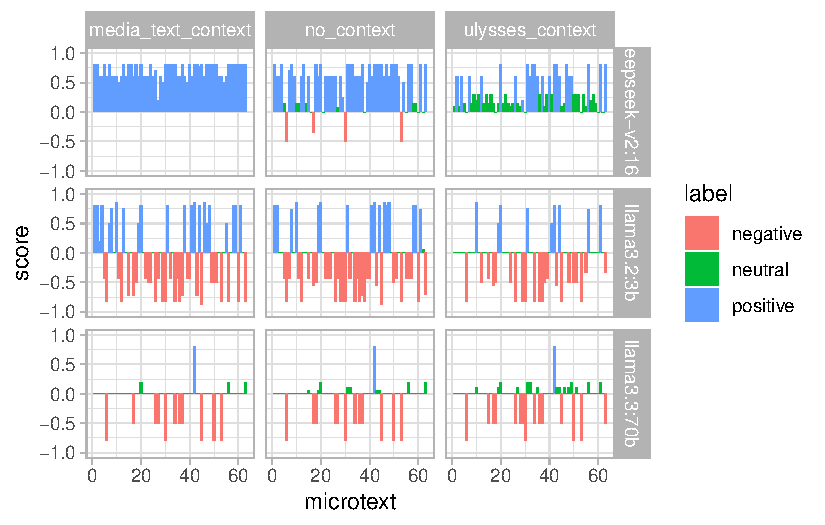
\includegraphics[keepaspectratio]{index_files/figure-pdf/fig-microtext-granularity-1.pdf}}

}

\caption{\label{fig-microtext-granularity}The three models disagreed
substantially about the sentiments of many microtexts, and showed
varying robustness to different prompts.}

\end{figure}%

\textsubscript{Source:
\href{https://uom-digital-studies.github.io/aeolus-microtexts/index.qmd.html}{Article
Notebook}}

\protect\phantomsection\label{cell-fig-sentence-aggregation}
\begin{figure}[H]

\centering{

\pandocbounded{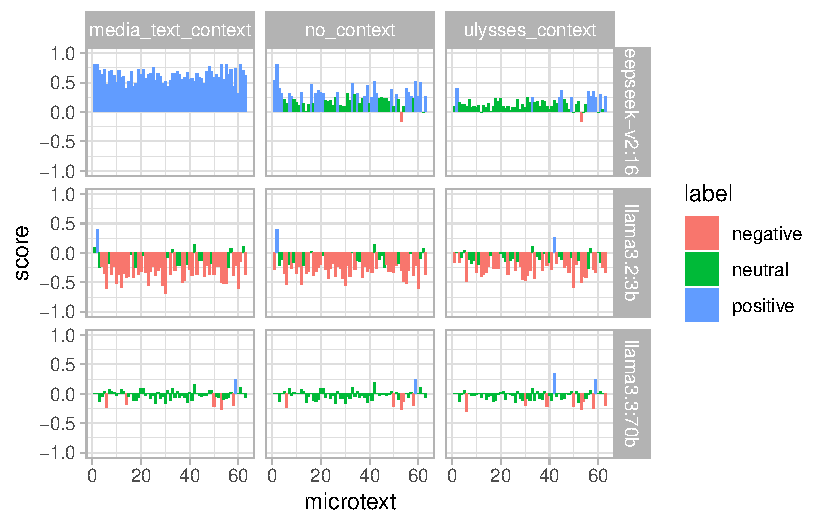
\includegraphics[keepaspectratio]{index_files/figure-pdf/fig-sentence-aggregation-1.pdf}}

}

\caption{\label{fig-sentence-aggregation}Segmenting the microtexts by
sentence, then averaging the LLMs scores across sentences, produced
substantially different results for all models.}

\end{figure}%

\textsubscript{Source:
\href{https://uom-digital-studies.github.io/aeolus-microtexts/index.qmd.html}{Article
Notebook}}

The three models have remarkably different biases:
\texttt{deepseek-v2:16b} has a strong positive bias;
\texttt{llama3.2:3b} tends to give extreme scores to all texts; and
\texttt{llama3.3:70b} is highly discriminative, giving extreme scores to
some texts and neutral scores to most.

The three models also vary in their response to the contextual clues.
For clarity, the three contextual clues injected into the prompt were:

\begin{itemize}
\tightlist
\item
  \texttt{media\_text\_context}: ``This text is, or is intended to
  resemble, social media content.''
\item
  \texttt{ulysses\_context}: ``This text is from James Joyce's novel
  Ulysses.''
\item
  \texttt{no\_context}: {[}No text injected to describe the text to be
  classified.{]}
\end{itemize}

The three models also give remarkably different results based on the
segmentation of the text. This is also a problem in traditional
sentiment analysis, but to a much lesser degree. In traditional
sentiment analysis, each word is scored deterministically, and then the
researcher chooses how to aggregate the word-level scores. In LLM-based
sentiment analysis, the text is scored as a whole; different
segmentations lead to incommensurable scores, which are therefore hard
to aggregate.

All models showed some sensitivity to this changes, but
\texttt{deepseek-v2:16b} showed especial sensitivity. For example, when
asked to score each microtext as a complete unit, it never gave a
negative score except when no contextual clue was injected into the
prompt.

\section{Validation: Lexicon-based sentiment
analysis}\label{sec-validation}

\textsubscript{Source:
\href{https://uom-digital-studies.github.io/aeolus-microtexts/index.qmd.html}{Article
Notebook}}

Like the LLM-analysis, the sentiment lexicons are inconsistent
(Figure~\ref{fig-lexicon-scores}; Table~\ref{tbl-consensus}). Overall,
the lexicons appear to agree most with \texttt{deepseek-v2:16b}, which
is however the least reliable of the LLMs that we tried, having the
worst calibration and prompt sensitivity. Despite this confusing overall
picture, however, the lexicon-based analysis has significant advantages
over the LLM-based analysis when we turn to close reading of the
passages, as we show in Section~\ref{sec-interpretation}.

\protect\phantomsection\label{cell-fig-lexicon-scores}
\begin{figure}[H]

\centering{

\pandocbounded{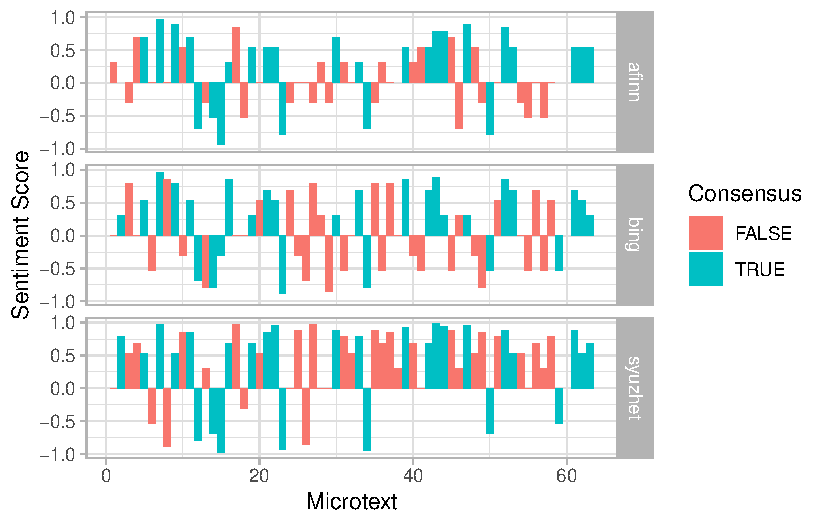
\includegraphics[keepaspectratio]{index_files/figure-pdf/fig-lexicon-scores-1.pdf}}

}

\caption{\label{fig-lexicon-scores}The three sentiment lexicons disagree
about the polarity of more than half the microtexts. \texttt{Consensus}
means all three lexicons agree on the overall positivity or negativity
of the microtext.}

\end{figure}%

\textsubscript{Source:
\href{https://uom-digital-studies.github.io/aeolus-microtexts/index.qmd.html}{Article
Notebook}}

\begin{longtable}[]{@{}lrl@{}}

\caption{\label{tbl-consensus}The sentiment lexicons agree on fewer than
half the microtexts.}

\tabularnewline

\toprule\noalign{}
Consensus & Microtexts & Proportion \\
\midrule\noalign{}
\endhead
\bottomrule\noalign{}
\endlastfoot
FALSE & 34 & 54.8\% \\
TRUE & 28 & 45.2\% \\

\end{longtable}

\textsubscript{Source:
\href{https://uom-digital-studies.github.io/aeolus-microtexts/index.qmd.html}{Article
Notebook}}

\section{Interpretation: Microtext \#45}\label{sec-interpretation}

\textsubscript{Source:
\href{https://uom-digital-studies.github.io/aeolus-microtexts/index.qmd.html}{Article
Notebook}}

How can this analysis actually assist close reading? In this
presentation, we briefly consider the case of Microtext \#45
(Figure~\ref{fig-close-reading}). \#45 is an especially interesting
section of `Aelous' for two reasons. First, one of the characters
expresses---or rather quotes---virulent nationalist and anti-Semitic
sentiments. Second, it is the only part of \emph{Ulysses} for which we
possess a recording in James Joyce's voice.

\begin{figure}

\begin{minipage}[t]{0.50\linewidth}

\centering{

\pandocbounded{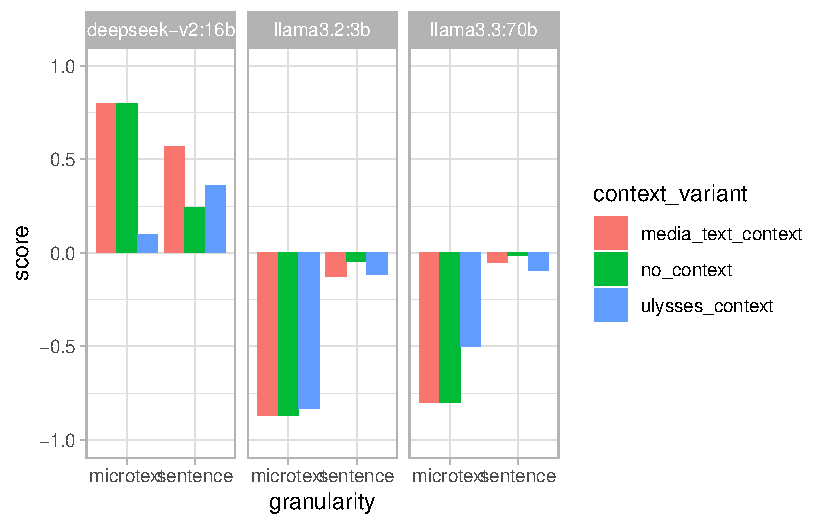
\includegraphics[keepaspectratio]{index_files/figure-pdf/fig-close-reading-1.pdf}}

}

\subcaption{\label{fig-close-reading-1}LLM scores}

\end{minipage}%
%
\begin{minipage}[t]{0.50\linewidth}

\centering{

\pandocbounded{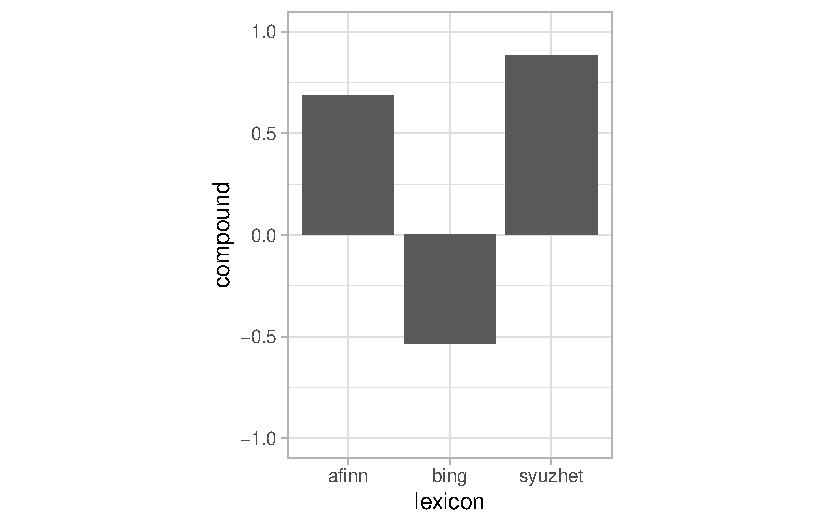
\includegraphics[keepaspectratio]{index_files/figure-pdf/fig-close-reading-2.pdf}}

}

\subcaption{\label{fig-close-reading-2}Lexicon scores}

\end{minipage}%

\caption{\label{fig-close-reading}Sentiment scores for Microtext \#45.}

\end{figure}%

In our perspective, Microtext \#45 does not have a strong emotional
polarity. It certainly contains negative sentiments, but these are
refracted through quotation. The microtext has four main components: the
headline (``FROM THE FATHERS''); one character's inner monologue
(Stephen's); another character's recitation of a nationalist,
anti-Semitic speech printed in the newspaper (J. J. O'Molloy reciting
John F. Taylor); and the narrator's bemused comments on the action.

As we will show in the presentation, out initial LLM results give us few
clues about how to interpret the texture of this passage. They give the
entire microtext a score, without any clues as to what features of the
text have influenced the score. By contrast, the lexicon-based approach
immediately draws the reader's attention to sentiment-laden words
(Table~\ref{tbl-45-words}), which provides a basis for critical
discussion. Which words are identified as sentiment-laden? Is this
machine judgment reasonable in the context of the microtext? How do
these judgements prompt us to re-read the passage?

\begin{longtable}[]{@{}lrlll@{}}

\caption{\label{tbl-45-words}The sentiment-laden words identified by the
three lexicons in Microtext \#45.}

\tabularnewline

\toprule\noalign{}
word & n & afinn & bing & syuzhet \\
\midrule\noalign{}
\endhead
\bottomrule\noalign{}
\endlastfoot
accept & 1 & positive & NA & positive \\
accepted & 1 & positive & NA & positive \\
admonition & 1 & NA & negative & negative \\
arrogant & 1 & negative & negative & negative \\
awe & 1 & NA & positive & NA \\
boldly & 1 & positive & NA & positive \\
bondage & 1 & NA & negative & negative \\
bowed & 3 & NA & NA & negative \\
child & 1 & NA & NA & positive \\
chosen & 1 & NA & NA & positive \\
cloud & 1 & NA & negative & negative \\
combat & 1 & negative & NA & negative \\
corrupted & 2 & NA & negative & negative \\
cradle & 1 & NA & NA & positive \\
culture & 1 & NA & NA & positive \\
curse & 1 & negative & negative & negative \\
dumb & 1 & negative & negative & negative \\
effigy & 1 & NA & negative & NA \\
enjoying & 1 & positive & positive & positive \\
good & 3 & positive & positive & positive \\
humanity & 1 & NA & NA & positive \\
hunger & 1 & negative & NA & negative \\
idol & 1 & NA & positive & positive \\
inspiration & 1 & positive & positive & positive \\
laden & 1 & NA & NA & negative \\
majestic & 1 & NA & positive & positive \\
mighty & 1 & NA & positive & positive \\
mysterious & 1 & NA & negative & negative \\
no & 2 & negative & NA & NA \\
obscure & 1 & NA & negative & negative \\
outlaw & 1 & NA & negative & negative \\
pray & 1 & positive & NA & positive \\
priesthood & 1 & NA & NA & positive \\
primitive & 1 & NA & negative & negative \\
saint & 1 & NA & positive & positive \\
shining & 1 & NA & NA & positive \\
speech & 1 & NA & NA & positive \\
spirit & 1 & positive & NA & positive \\
supple & 1 & NA & positive & positive \\
supremely & 1 & NA & positive & positive \\
terrible & 1 & negative & negative & negative \\
weak & 1 & negative & negative & negative \\
wealth & 1 & positive & NA & positive \\
youthful & 1 & positive & positive & positive \\

\end{longtable}

\textsubscript{Source:
\href{https://uom-digital-studies.github.io/aeolus-microtexts/index.qmd.html}{Article
Notebook}}

\section{Conclusion: Next Steps}\label{conclusion-next-steps}

This is a work-in-progress presentation, so we conclude with our plans
for future work. We have 3 key plans:

\begin{enumerate}
\def\labelenumi{\arabic{enumi}.}
\tightlist
\item
  Repeat the experiments with larger and more recent LLMs, now that we
  have access to a more recent version of Ollama. We expect that larger
  and more capable models will be more reliable, though there are good
  reasons to doubt this.
\item
  Include a ``reasoning'' field in the research question schemas, so
  that LLMs are obliged to provide a rationale for their scores. This
  may increase the interpretability of the results, thus making them
  more useful for close reading.
\item
  Construct a dataset of human scores to for a third point of
  validation.
\item
  Quantify our notions of ``calibration,'' ``discrimination'' and
  ``prompt sensitivity'' (adapting Rabanser et al. (2026)) to help
  develop a shared computational language for evaluating LLM research
  assistants.
\end{enumerate}

In the long run, LLMs will only be useful for literary criticism if they
can be effectively harnessed to enrich our subjective experience of
texts. This new technology has not altered the fundamental aim of
algorithmic criticism: to ``channel the heightened objectivity made
possible by the machine into the cultivation of those heightened
subjectivities necessary for critical work'' (Ramsay 2011, ix).

\section{Appendices}\label{appendices}

\subsection{Appendix 1: Nationalism and User-Generated
Content}\label{sec-other-rqs}

In addition to sentiment analysis, we also performed thematic analysis
using the LLMs. Initial results are shown here for interest.

The second task we gave the LLMs was: Classify the nationalist
orientation of this text. Results were similar to the sentiment analysis
questions. All the models showed good calibration (the numerical score
corresponded to the label given by the model), but varied in their
prompt sensitivity and judgments.

\protect\phantomsection\label{cell-fig-nationalism-microtext}
\begin{figure}[H]

\centering{

\pandocbounded{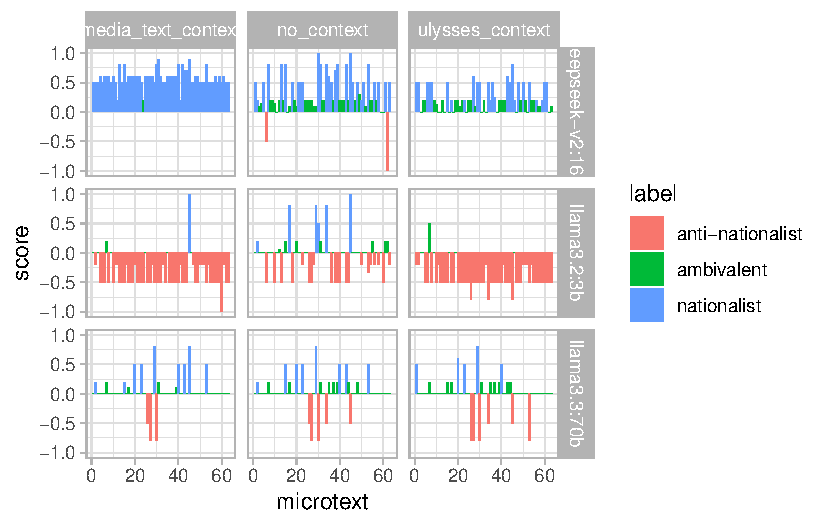
\includegraphics[keepaspectratio]{index_files/figure-pdf/fig-nationalism-microtext-1.pdf}}

}

\caption{\label{fig-nationalism-microtext}The nationalism research
question shows a similar distribution of results to the sentiment
analysis question.}

\end{figure}%

\textsubscript{Source:
\href{https://uom-digital-studies.github.io/aeolus-microtexts/index.qmd.html}{Article
Notebook}}

\protect\phantomsection\label{cell-fig-nationalism-sentence}
\begin{figure}[H]

\centering{

\pandocbounded{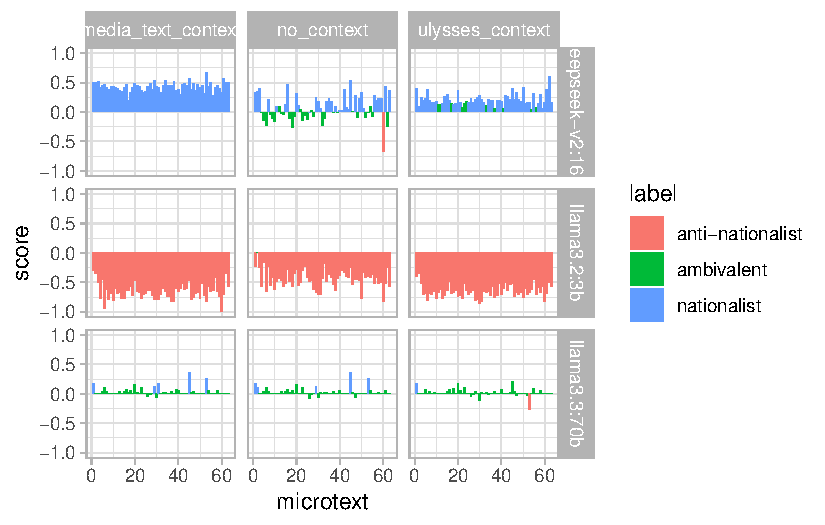
\includegraphics[keepaspectratio]{index_files/figure-pdf/fig-nationalism-sentence-1.pdf}}

}

\caption{\label{fig-nationalism-sentence}As with sentiment analysis,
analysing by sentence and then aggregating produces starkly different
results.}

\end{figure}%

\textsubscript{Source:
\href{https://uom-digital-studies.github.io/aeolus-microtexts/index.qmd.html}{Article
Notebook}}

The third task we gave the LLMs was: Judge the resemblance of this text
to typical user-generated content. Here the two smaller models failed.
Their calibration was maximally poor: they labelled every microtext as
``ugc'' even if awarding a negative score. This poor calibration was
repeated when the LLMs analysed the microtexts on the sentence level.
The larger model showed good calibration and discrimination: the
`Aeolus' episode comments ironically on media discourse; the actual
fabric of the episode, with its dialogue and streams of consciousness,
rarely resembles media discourse on the surface.

The poor results may have been the fault of our research question
schema. Due to an oversight, the LLM was only given two labels to choose
from: \texttt{"ugc"} and \texttt{"other"}. There was no third label for
results in the middle of the scale. Since in our setup, the LLM outputs
the label before it outputs the numerical score, the numerical score
directly depends on the label. It is surprising that the calibration
between score and label was so poor on two of the models despite this.

\protect\phantomsection\label{cell-fig-ugc-microtexts}
\begin{figure}[H]

\centering{

\pandocbounded{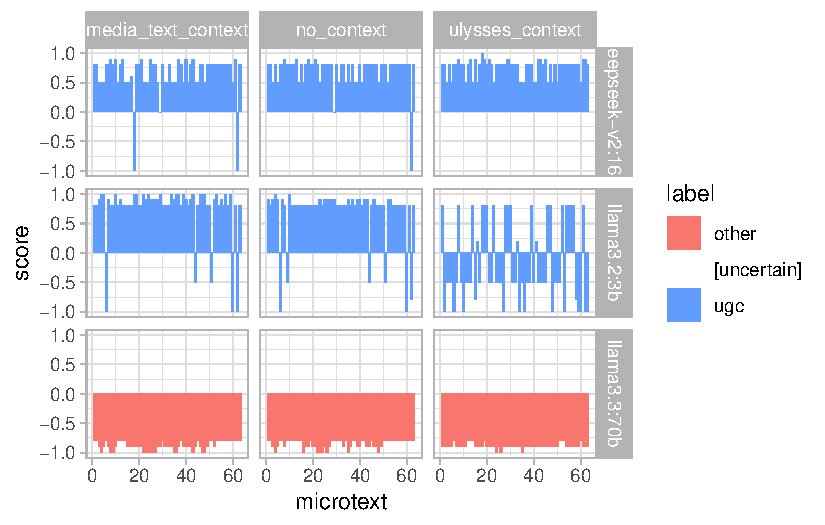
\includegraphics[keepaspectratio]{index_files/figure-pdf/fig-ugc-microtexts-1.pdf}}

}

\caption{\label{fig-ugc-microtexts}Results from the ``user-generated
content'' question are meaningless. NB: due to a flaw in our code, the
LLM was only provided two possible labels, unlike for the other
questions.}

\end{figure}%

\textsubscript{Source:
\href{https://uom-digital-studies.github.io/aeolus-microtexts/index.qmd.html}{Article
Notebook}}

\protect\phantomsection\label{cell-fig-ugc-sentences}
\begin{figure}[H]

\centering{

\pandocbounded{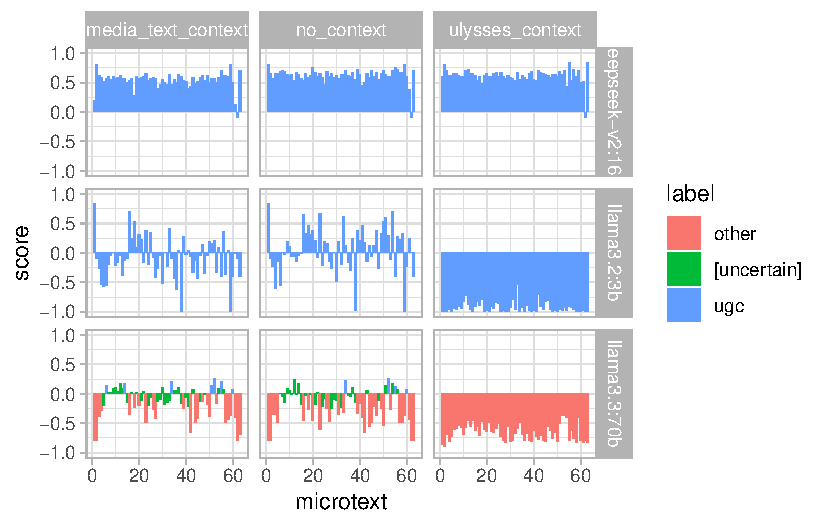
\includegraphics[keepaspectratio]{index_files/figure-pdf/fig-ugc-sentences-1.pdf}}

}

\caption{\label{fig-ugc-sentences}Sentence-level analysis also displays
very poor calibration on the smaller models. Note that the
`{[}uncertain{]}' label has been imputed from the aggregated
sentence-level scores.}

\end{figure}%

\textsubscript{Source:
\href{https://uom-digital-studies.github.io/aeolus-microtexts/index.qmd.html}{Article
Notebook}}

\subsection{Appendix 2: Normalising the lexicon-based sentiment
scores.}\label{appendix-2-normalising-the-lexicon-based-sentiment-scores.}

The LLMs were asked to score the microtexts between -1 and 1 on all
three tasks. To compare these LLM scores with the lexicon-based scores,
we therefore converted the lexicon-based scores to a numerical scale. We
adapted the method of Hutto and Gilbert (2014), shown in
Equation~\ref{eq-vader-normalisation}.

\begin{equation}\protect\phantomsection\label{eq-vader-normalisation}{
compound = \frac{sum(pos) + sum(neg)}{\sqrt{(sum(pos) + sum(neg))^2 + \alpha}}
}\end{equation}

Where \(pos\) is the sum of positively-scored words in the text, \(neg\)
is the sum of negatively-scored words, and \(\alpha\) is the expected
maximum score for a given text. VADER gives a score between -4 and 4 for
each word, and is calibrated to short social media texts such as tweets.
They empirically determined \(\alpha\) to be \(15\). Since two of our
lexicons, \emph{bing} and \emph{afinn}, simply give a text label to each
word (\texttt{"positive"} or \texttt{"negative"}), we determined
\(\alpha\) differently. We convert the labels to a \(-1\) and \(1\), and
then inspect the distribution (Figure~\ref{fig-classic-scores-dist}).
Although \emph{syuzhet} occasionally returns more extreme scores, we
determine \(10\) as the most appropriate value for \(\alpha\) on our
scale.

\protect\phantomsection\label{cell-fig-classic-scores-dist}
\begin{figure}[H]

\centering{

\pandocbounded{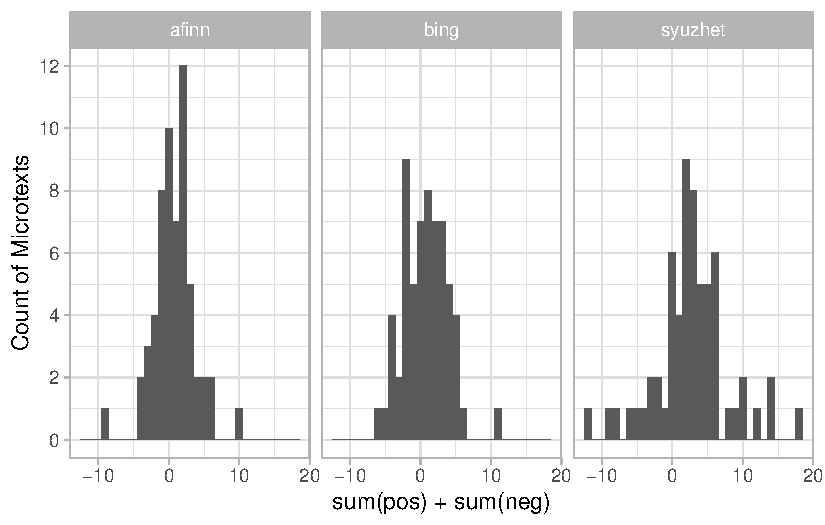
\includegraphics[keepaspectratio]{index_files/figure-pdf/fig-classic-scores-dist-1.pdf}}

}

\caption{\label{fig-classic-scores-dist}Most texts achieve a score
between -10 and 10 on inspection of the histogram.}

\end{figure}%

\textsubscript{Source:
\href{https://uom-digital-studies.github.io/aeolus-microtexts/index.qmd.html}{Article
Notebook}}

\section{AI Declaration}\label{ai-declaration}

We used Posit Assistant to assist writing the orchestration code and to
document our design decisions for the research compendium. All
agent-facing documentation is available in the Github repository for
this project in the \texttt{docs/} directory or the project root. The
code in this abstract was hand-written, with occasional recourse to AI
to help identify bugs. All code in the project, whether handwritten or
drafted with AI assistance, has been reviewed line-by-line by a human,
and we take full responsibility for every line.

All prose in this abstract was human-authored without exception.

\section*{References}\label{references}
\addcontentsline{toc}{section}{References}

\protect\phantomsection\label{refs}
\begin{CSLReferences}{1}{1}
\bibitem[\citeproctext]{ref-barke_agents_2026}
Barke, Shraddha, and Adithya Murali. 2026. {``Agents as {Software}: {A}
{Programming} {Languages} {Agenda} for {Agent} {Reliability}.''}
\emph{Proceedings of the 2026 {ACM} {SIGPLAN} {International}
{Symposium} on {New} {Ideas}, {New} {Paradigms}, and {Reflections} on
{Programming} and {Software}} (New York, NY, USA), Onward! '26, October,
179--90. \url{https://doi.org/10.1145/3840586.3843744}.

\bibitem[\citeproctext]{ref-elkins_shapes_2022}
Elkins, Katherine. 2022. \emph{The {Shapes} of {Stories}: {Sentiment}
{Analysis} for {Narrative}}. Cambridge University Press.
\url{https://doi.org/10.1017/9781009270403}.

\bibitem[\citeproctext]{ref-falk_romanticism_2024}
Falk, Michael. 2024. \emph{Romanticism and the {Contingent} {Self}:
{The} {Challenge} of {Representation}}. Palgrave {Studies} in the
{Enlightenment}, {Romanticism} and {Cultures} of {Print}. Springer
International Publishing.
\url{https://doi.org/10.1007/978-3-031-49959-3}.

\bibitem[\citeproctext]{ref-franta_sentiment_2024}
Franta, Andrew, and Sean Silver. 2024. {``Sentiment {Analysis} and the
{Sentimental} {Novel}.''} \emph{Critical Inquiry} 50 (3): 402--24.
\url{https://doi.org/10.1086/728948}.

\bibitem[\citeproctext]{ref-goebel_explainable_2018}
Goebel, Randy, Ajay Chander, Katharina Holzinger, et al. 2018.
{``Explainable {AI}: {The} {New} 42?''} In \emph{Machine {Learning} and
{Knowledge} {Extraction}}, edited by Andreas Holzinger, Peter Kieseberg,
A Min Tjoa, and Edgar Weippl. Lecture {Notes} in {Computer} {Science}.
Springer International Publishing.
\url{https://doi.org/10.1007/978-3-319-99740-7_21}.

\bibitem[\citeproctext]{ref-hu_mining_2004}
Hu, Minqing, and Bing Liu. 2004. {``Mining and Summarizing Customer
Reviews.''} \emph{Proceedings of the Tenth {ACM} {SIGKDD} International
Conference on {Knowledge} Discovery and Data Mining} (New York, NY,
USA), {KDD} '04, August, 168--77.
\url{https://doi.org/10.1145/1014052.1014073}.

\bibitem[\citeproctext]{ref-hutto_vader_2014}
Hutto, C., and Eric Gilbert. 2014. {``{VADER}: {A} {Parsimonious}
{Rule}-{Based} {Model} for {Sentiment} {Analysis} of {Social} {Media}
{Text}.''} \emph{Proceedings of the International AAAI Conference on Web
and Social Media} 8 (1): 216--25.
\url{https://doi.org/10.1609/icwsm.v8i1.14550}.

\bibitem[\citeproctext]{ref-jockers_syuzhet_2015}
Jockers, Matthew. 2015. \emph{Syuzhet: {Extract} {Sentiment} and {Plot}
{Arcs} from {Text}}. \url{https://github.com/mjockers/syuzhet}.

\bibitem[\citeproctext]{ref-kim_sentiment_2022}
Kim, Hoyeol. 2022. {``Sentiment {Analysis}: {Limits} and {Progress} of
the {Syuzhet} {Package} and {Its} {Lexicons}.''} \emph{Digital
Humanities Quarterly} 016 (2).

\bibitem[\citeproctext]{ref-lawrence_aeolus_1980}
Lawrence, Karen R. 1980. {``"{Aeolus}": {Interruption} and
{Inventory}.''} \emph{James Joyce Quarterly} 17 (4): 389--405.
\url{https://www.jstor.org/stable/25476319}.

\bibitem[\citeproctext]{ref-marwick_packaging_2018}
Marwick, Ben, Carl Boettiger, and Lincoln Mullen. 2018. {``Packaging
{Data} {Analytical} {Work} {Reproducibly} {Using} {R} (and
{Friends}).''} \emph{The American Statistician} 72 (1): 80--88.
\url{https://doi.org/10.1080/00031305.2017.1375986}.

\bibitem[\citeproctext]{ref-mcluhan_joyce_1954}
McLuhan, Marshall. 1954. {``Joyce, {Mallarmé}, and the {Press}.''}
\emph{The Sewanee Review} 62 (1): 38--55.
\url{https://www.jstor.org/stable/27538333}.

\bibitem[\citeproctext]{ref-mens_positioning_2025}
Mens, Gaël Le, and Aina Gallego. 2025. {``Positioning {Political}
{Texts} with {Large} {Language} {Models} by {Asking} and {Averaging}.''}
\emph{Political Analysis} 33 (3): 274--82.
\url{https://doi.org/10.1017/pan.2024.29}.

\bibitem[\citeproctext]{ref-nielsen_new_2011}
Nielsen, Finn Årup. 2011. {``A New {ANEW}: {Evaluation} of a Word List
for Sentiment Analysis in Microblogs.''} \emph{CoRR} abs/1103.2903.
\url{https://doi.org/10.48550/ARXIV.1103.2903}.

\bibitem[\citeproctext]{ref-ornstein_how_2025}
Ornstein, Joseph T., Elise N. Blasingame, and Jake S. Truscott. 2025.
{``How to Train Your Stochastic Parrot: Large Language Models for
Political Texts.''} \emph{Political Science Research and Methods} 13
(2): 264--81. \url{https://doi.org/10.1017/psrm.2024.64}.

\bibitem[\citeproctext]{ref-rabanser_towards_2026}
Rabanser, Stephan, Sayash Kapoor, Peter Kirgis, Kangheng Liu, Saiteja
Utpala, and Arvind Narayanan. 2026. \emph{Towards a {Science} of {AI}
{Agent} {Reliability}}. arXiv.
\url{https://doi.org/10.48550/arXiv.2602.16666}.

\bibitem[\citeproctext]{ref-radak_aeolus_2017}
Radak, Tamara. 2017. {``"{Aeolus}'', {Interrupted}: {Heady} {Headlines}
and {Joycean} {Negotiations} of {Closure}.''} In \emph{Publishing in
{Joyce}'s \emph{Ulysses}}, edited by William Brockman, Tekla Mecsnóber,
and Sabrina Alonso. BRILL.
\url{https://doi.org/10.1163/9789004359062_011}.

\bibitem[\citeproctext]{ref-ramsay_reading_2011}
Ramsay, Stephen. 2011. \emph{Reading {Machines}: {Towards} an
{Algorithmic} {Criticism}}. University of Illinois Press.

\bibitem[\citeproctext]{ref-schneider_mediatization_1989}
Schneider, Ulrich. 1989. {``Mediatization in "{Aeolus}" and "{Oxen} of
the {Sun}".''} \emph{European Joyce Studies} 1: 15--21.
\url{https://www.jstor.org/stable/44871172}.

\bibitem[\citeproctext]{ref-openai_structured_data_docs}
{``Structured Model Outputs {\textbar} {OpenAI} {API}.''} n.d. In
\emph{OpenAI Developers}. Accessed November 11, 2026.
\url{https://developers.openai.com/api/docs/guides/structured-outputs}.

\end{CSLReferences}




\end{document}
